%[prl] it will mess up section numbers but puts our emails in the bibliography section
%[eqsecnum] Number equations by section
\documentclass[aps,prb,twocolumn,superscriptaddress]{revtex4-1}
\usepackage{graphicx}  % this is the up-to-date package for all figures
\usepackage{amssymb}   % for math
\usepackage{verbatim}  % for the comment environment
\usepackage{color}
\usepackage{subcaption} % for subcaptions on side-by-side figures
\usepackage{float}	% allows use of 'H' command
\renewcommand{\thefootnote}{\roman{footnote}} %for footnotes in roman numerals

% This allows you to use '\cref{}' to reference sections with the symbol
\usepackage{cleveref}
\crefname{section}{\S}{\S\S}%{§}{§§}


%\usepackage{cite}	% to use .bib file
%\usepackage{hyperref}	% needed to add hyperlinks
%\hypersetup{
%  colorlinks=true,
%  linkcolor=blue,
%  filecolor=magenta,
%  urlcolor=cyan,
%}
\bibliographystyle{apsrev}

% For Numbered Sections---------------------------------------------------------------
% Usual (decimal) numbering
\renewcommand{\thesection}{\arabic{section}}
\renewcommand{\thesubsection}{\thesection.\arabic{subsection}}
\renewcommand{\thesubsubsection}{\thesubsection.\arabic{subsubsection}}
%% Fix references
%\makeatletter
%\renewcommand{\p@subsection}{}
%\renewcommand{\p@subsubsection}{}
%\makeatother
% ------------------------------------------------------------------------------------


% these are some custom control of the page size and margins
% \topmargin= 0.2in  % these 1st two may be needed for some computers
% \textheight=8.75in
\textwidth=6.5in
%\oddsidemargin=0cm
%\evensidemargin=0cm

% this is where the actual document itself (rather than control statements) begins:


\begin{document}



\title{Evaluating the Pan-STARRS Variability Parameter}


%\input author_list.tex

%\author{Daichi Hiramatsu\thanks{dhiramat@hawaii.edu}}
%\author{Corey Muntik\thanks{cmutnik@hawaii.edu}}

\author{Daichi Hiramatsu}
\email{dhiramat@hawaii.edu}
\author{Corey Mutnik}
\email{cmutnik@hawaii.edu}
\affiliation{Department of Physics \& Astronomy, \\
University of Hawai`i at M\={a}noa}
%\affiliation{Department of Physics \& Astronomy, \\University of Hawaii at Manoa,\\2505 Correa Rd, Honolulu, HI, 96822, USA}
%\altaffiliation{Observational Astronomy 301}



\begin{abstract}
\textbf{By Thursday (4/18) we need:} well thought out section titles and plots that show all the points we wanna make\\

remake prob(f) plot with all 300,000 stars (not only 80,000)\\

LS analysis on ATLAS Pathfinder Telescope data, verified PS variability criteria
\end{abstract}

\maketitle    




\section{Introduction}


\begin{itemize}
	\item{} why we care
	\item{} what made us care about this project
	\item{} NO structure $/$ distance stuff (maybe put it in looking forward section at end)
	\item{} talk about PS catalog
	\item{} variability surveys (discuss other attempts to measure variables across the sky)
	\item{} why are variables interesting
	%\item{} why do we want to find variables and care about where they are located
	\item{} Summary: we ran LS, analyzed stars, why did we do it all
	\item{} Mention what will be discussed: ``in section 2 we describe the observations we used...''
\end{itemize}



\section{ATLAS Pathfinder Observations}


We used the $0.18$~m Asteroid Terrestrial-impact Last Alert System (ATLAS) Pathfinder telescope~\citep{fallingstar} at the Mauna Loa. The field of view (FOV) of the telescope is $5.2^{\circ}$ with the angular resolution (effective PSF FWHM) of $5$". Thanks to its wide FOV, it is suitable for our project, wide field study. The spatial resolution, however, is not great. For this reason, we chose our field to be slightly off the galactic plane. 



\subsection{SNR Calculation}\label{sec:SNR}

To calculate an appropriate sampling frequency and SNR, typical RR Lyrae light curves~\cite{RRLyrae} were used with artificially introduced gaps and noise following the Gaussian distribution. To determine distances from the PL relations~\citep{PL} within $\simeq5\%$ accuracy assuming typical metalicity $Z=0.001$, we need periods within $\simeq1\%$ accuracy. The period range of RR Lyrae stars is $0.05$ to $1.2$ days ~\cite{Astro} which contrains the sampling frequency. By using the Lomb-Scargle analysis (discussed in \cref{sec:PA}), it was found that 15 nights with 10 observations/night is the lower limit sampling duration and rate to achieve the desired period accuracy. Since the magnitude fluctuations of RR Lyrae are typically in the range of $0.3$ to $2.0$ mags ~\cite{AAVSO}, the uncertainty in magnitude was taken to be $0.1$ mags, and the changes, $0.01$ to $0.1$ mags, in the uncertainty did not affect the period determinations significantly. Thus we only needed $10\%$ photometry. For $m_g = m_r = 16$ and $m_i = 15.7$, an exposure time of $20$~sec yields $10\%$ photometry for the ATLAS pathfinder telescope~\citep{fallingstar}.



\begin{itemize}
	\item{} we used data from ATLAS
	\item{} supplemented with ATLAS data [REF TONRY] (possibly make this s subsection)
%	\item{} exposure time
%	\item{} observation dates
	\item{} what was the weather like during observations
	\item{} PSF FWHM variations (only include if we discuss crowding)
	\item{} `we recieved the reduced image data from the ATLAS pipeline; which gave us RA, Dec, mag, etc...'
	\item{}\url{http://fallingstar.com/how_atlas_works.php}
\end{itemize}


~[VERIFY CORRECT CITATIONS:\\% $http://rsta.royalsocietypublishing.org/content/371/1992/20120269$]\\
%In determining the variability of stars in our FOV, data from the $gri Project$~\cite{gri} was used.\\
Initially, determination of variability was going to be achieved using data collected by the $gri Project$~\cite{gri}.  The $gri Project$ is [EXPLAIN]...\\
In order to reduce aliasing, extra observations needed to be made.  Observation procedures are discussed in~\cref{sec:data}.
~[PATHFINDER USED FOR GRI DATA...the reduction process is discussed at length Tonry in...cite]\\
We received the reduced image data from the ATLAS pipeline~\cite{PSpipe}~\cite{tonrypipe}
%\cite{PSimgpipe,*tonrypipe}



\subsection{Data Collection}\label{sec:data}
%\begin{itemize}
%	\item{} how we got mags out of data...
%	\item{} $l^{II}=202^{\circ}$
%	\item{} $b^{II}=\pm5$
%\end{itemize}
% from old paper
\iffalse
	\begin{itemize}
	 \item{} split observations into 1 $deg^2$ chunks
	 \item{} isolated groups s.t. each one is a star with 12 or more obs
	 \item{} $--$ more than 12 detections to be a star
	 \item{} $--$ any sq deg that has more than one star
	 \item{} this reduced 1300 $deg^2$ observation data down to ~300
	 \item{} before variability params: 1531417 stars in field
	 \item{} for variability parameters
	 \item{} $--$ log(average(upper quartile)) - log(average(lower quartile))
	 \item{} $--$ expect variation to go at .2* mag (from sqrt noise)...so subtract .2mag to get the logritmic statistic
	 \item{} sorted biggest (most variable?) to smallest (least variable?)
%	 \item{} ran FLS on 80,000 most variable stars, rather than full star groupings (over 1million)
	\end{itemize}
\fi

~[NEED TO CITE TONRY FOR OUR OBSERVATIONS]\\
~[MENTION THAT OUR OBS NECESSARY TO REDUCE ALIASING]\\

Using the Pathfinder telescope, observations were made at two galactic latitudes ($b^{II}=\pm5^{\circ}$) and spanned a range of galactic longitudes ($202^{\circ} < l^{II} < 232^{\circ}$).  Observations discussed here indicated the center of each FOV.  
Exposures were collected for 20~s and separated by $3^{\circ}$ longitudinally.  For implementation by the Pathfinder telescope, a conversion to RA and Dec was made; giving a range of $93 < RA < 119^{\circ}$ and $-20^{\circ} < Dec < 13^{\circ}$, as shown by Figure~\ref{fig:simoverlap}.  To account for the 0.05~$^{\circ}$ gap between the detectors, a 0.1~$^{\circ}$ offset in RA was implemented on every other night.  
%Ten observations per night were collected for 20 nights, spanning 3/8/16-3/27/16.
%Observations were collected between 3/8/16-3/27/16.  During this 20 day period, we collected 10 observations per night.  
Spanning 20 nights, 10 observations a night were collected on 3/8/16-3/27/16.  Luckily, all of these nights had weather perfectly attuned for observations.  Half a night of observations were lost on 3/19/26, due to a crash of the server controlling the telescope.


%0.1 deg offset in RA, accounts for 0.05 deg gap between the two detectors.
%~\\~[dRA = dangle / cos(Dec)]
Observations were traced out by moving the FOV by $3^{\circ}$ longitudinally, starting at $b^{II}=-5^{\circ}$, $l^{II}=202^{\circ}$ and ending at $b^{II}=-5^{\circ}$, $l^{II}=232^{\circ}$.  Once observations at $b^{II}=-5^{\circ}$ were complete, the FOV was shifted to $b^{II}=+5^{\circ}$, $l^{II}=232^{\circ}$.
%Observations were traced out by taking the first exposure at $b^{II}=-5^{\circ}$ and $l^{II}=202^{\circ}$, moving the FOV longitudinally by $3^{\circ}$
%Starting at $b^{II}=-5^{\circ}$ and $l^{II}=202^{\circ}$, exposures were collected for 20~s
%Observations were made by starting at $b^{II}=-5^{\circ}$ and $l^{II}=202^{\circ}$, moving the ...Each exposure was collected for 20
%Data was collected for \\
%Starting at $b^{II}=-5^{\circ}$ and $l^{II}=202^{\circ}$ \\
%20~s exposures were collected\\


%\begin{figure}[H]
%	\centering
%	%\caption{prob(f)}
%	\textbf{Sorting Pattern}\par\medskip
%		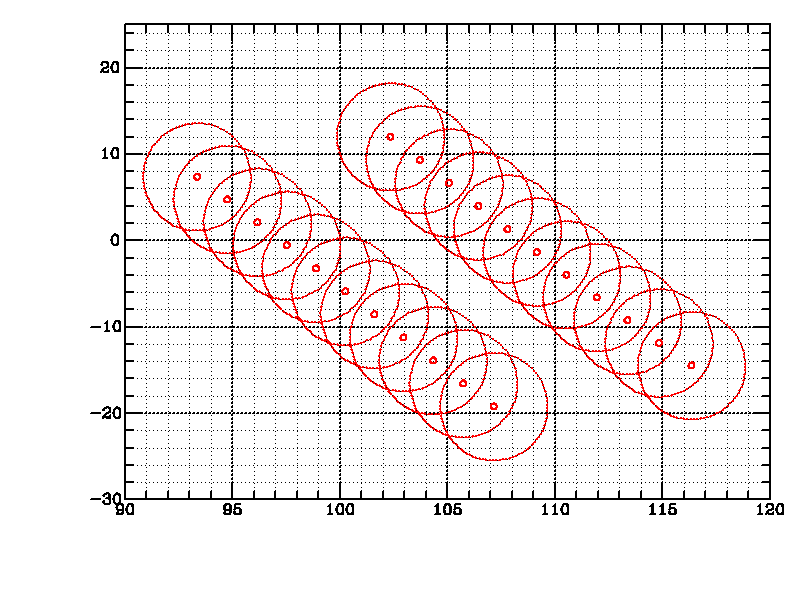
\includegraphics[width=3.35in]{figures/fromJT/sortedFOV.png}
%	\caption{\it \small{Stars were grouped in the pattern shown (down the collected observations)}}
%	\label{fig:sortpat}
%\end{figure}



\subsection{Object Cuts}\label{sec:cuts}

Various data points, reduced by the ATLAS pipeline~\cite{gri}, were returned with magnitude errors of zero.  Such 
values were not used determining variability of the source.  In order for an identified star to be considered for 
variability testing, we required a minimum of 12 ``good'' observations.  A ``good'' detection is meets the minimum 
PSF, does not fall on the edge of each $1~deg^{2}$ FOV, and was observed with clear skies.  A minimum of 12 
observations was deemed necessary, in order to eliminate aliasing, as discussed in~\cref{sec:PA}.  After observation 
cuts were applied, 1.5 Billion stars remained in our FOV.  


\begin{figure}[H]
 \centering
 	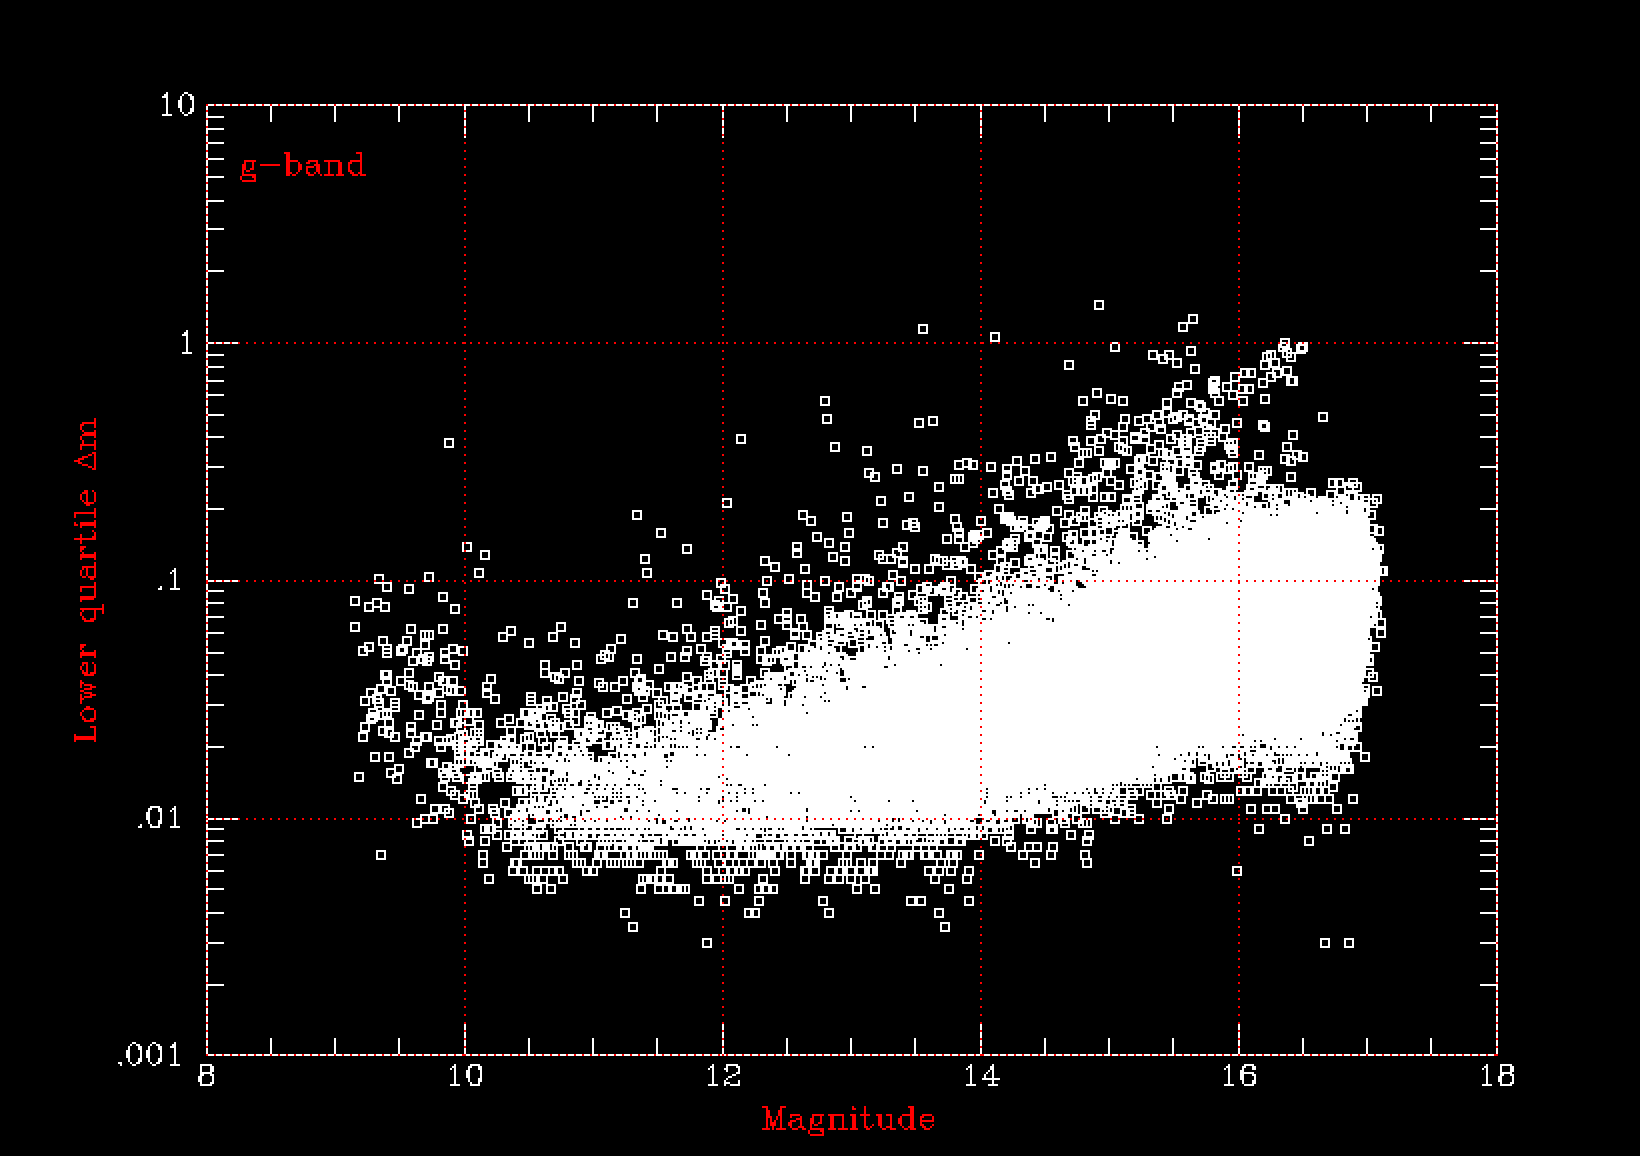
\includegraphics[width=3.35in]{figures/scatter_gfilt_57452_57455.png}
 \caption{\it \small{Lower quartile variance as a function of magnitude.}}
 \label{fig:probrrHPS}
\end{figure}
  In order to exploit the lower quartile variance, shown in Figure~\ref{fig:quart}, a factor of $0.2m$ was added to account for Poisson error.  
The higher a star deviates from the average value, the more likely it is variable.  


%______________
As a result of running FLS, the most variable candidates fell below $logPr(rnd)= -45$, shown in Figure~\ref{fig:logPr}.  

%______________


~[DESCRIBE logPr(rnd)...how some vars might have slipped past, but only ]\\
~[CITE WHERE IT SAYS RRLYRAE HAVE 0.5 < PERIOD < 1.2 [DAYS]]\\



\iffalse
of all 1.5 billion stars in our FOV we scanned the most variable $(logPr(rnd)<=45)$\\
  - located: ${{{cd /home/rr_lyrae/logprob_below_neg45_take2}}}$\\
  - 1558 stars\\
new grouping list that DH wanted (after removing aliased regions)\\
  - located: ${{{cd /home/rr_lyrae/alias_rm_grps}}}$\\
  - 776 stars\\
\fi

\section{Constructing Stellar Light Curves}

% check out resource:
% https://www.aavso.org/lcg

\begin{itemize}
	\item{} how we selected stars (12+ obs, 1x1 deg$^2$, etc)
\end{itemize}

The selection process began


% merged these figures into side by side (below)
%\begin{figure}[H]
% \centering
% 	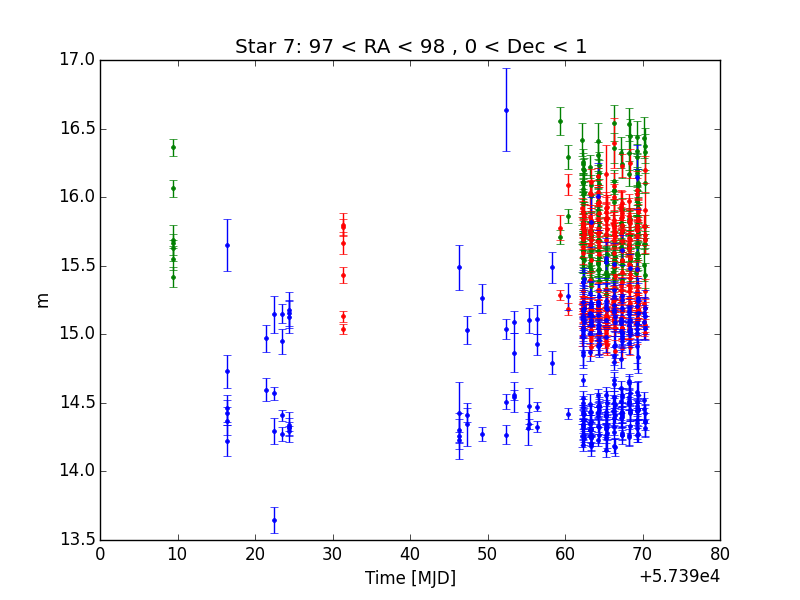
\includegraphics[width=3.35in]{figures/LC/star7_97_98_0_1.png}
% \caption{\it \small{Light Curve of variable star, using all collected and ATLAS data.}}
% \label{fig:LC7}
%\end{figure}
%\begin{figure}[H]
% \centering
% 	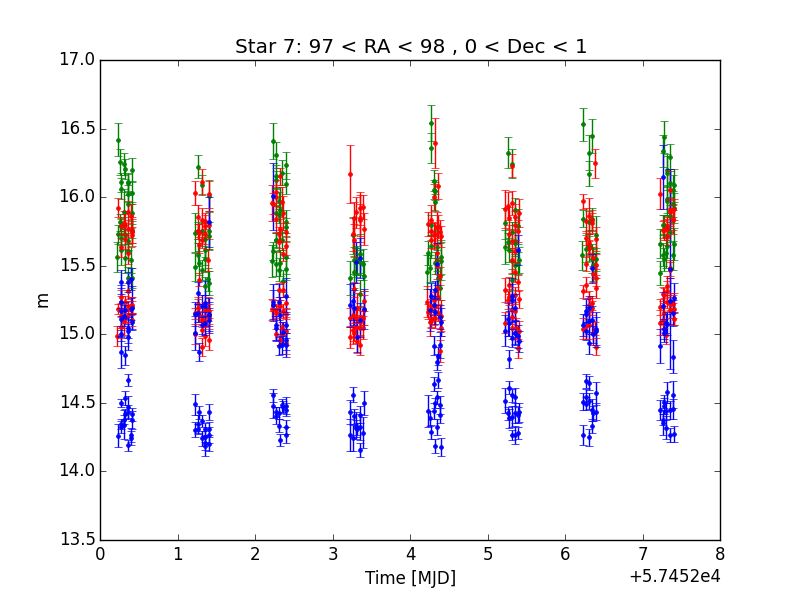
\includegraphics[width=3.35in]{figures/LC/star7_97_98_0_1_restricted.png}
% \caption{\it \small{Light Curve of variable star, using only collected data (without incorporating extra ATLAS data).}}
% \label{fig:restrictedLC7}
%\end{figure}



\begin{figure*}
	\centering
	\begin{subfigure}{.5\textwidth}
	  \centering
	  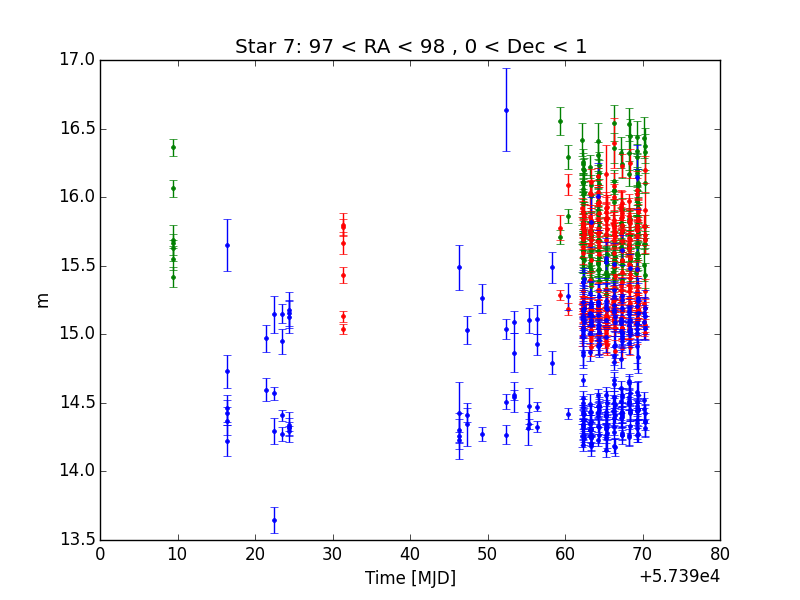
\includegraphics[width=1\linewidth]{figures/LC/star7_97_98_0_1.png}
		\caption{\it \small{ }}
		\label{fig:LC7}
	\end{subfigure}%
	\begin{subfigure}{.5\textwidth}
	  \centering
			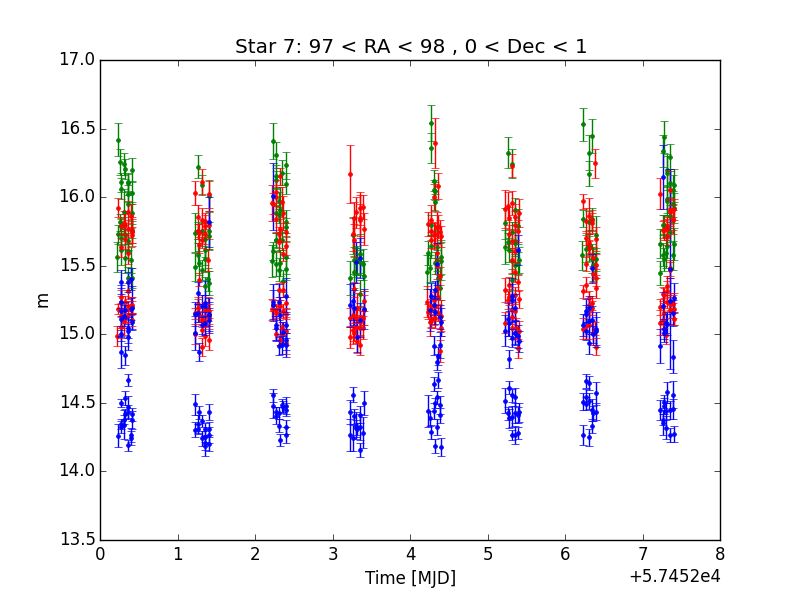
\includegraphics[width=1\linewidth]{figures/LC/star7_97_98_0_1_restricted.png}
		\caption{\it \small{ }}
		\label{fig:restrictedLC7}
	\end{subfigure}
	\caption{\it \small{Light Curve of a variable star.  Panel `(a)' shows a light curve constructed using all collected and ATLAS data.  Panel `(b)' is a restricted selection of `(a)', not showing any observations made by ATLAS.}}
	\label{fig:LC}
\end{figure*}



% clean up section title
\section{Periodogram Analysis}\label{sec:PA}

\iffalse
%------------- KILL subsection and make periodgram the intro to LS
%\subsection{Periodogram Analysis}
%\section{Identifying Variable Stars Using Lomb-Scargle}
~[INTRO TO WHAT IS PERIODOGRAM...WE CONSTRUCT PERGRAMS USING LS METHOD]
\begin{itemize}
	\item{} extract variability from LS
	\item{} describe how it works and why we used LS
	\item{} major aliasing at 1 day and 0.5 day periods
	\item{} things that fall at at -50 (in Figure~\ref{fig:quartiles}) means that those are VERY probably variable stars
	\item{} roughly \_\_\_\_\_ stars fell at -50 in Figure~\ref{fig:quartiles}
	\item{} 315,992 stars tested for variability
	\item{} other stars (outside of 315,992) are statistically unlikely to be variable
\end{itemize}
%-------------

\begin{itemize}
	\item{} brief explanation of the fast LS
	\item{} period search range to avoid aliasing
	\item{} compute gri periods individually and compare each other. if period differences are less than 0.04 days, next step
\end{itemize}
\fi


To extract periods from light curves, the Fast Fourier Transform (FFT) is usually used. For our data, however, FFT is not optimal due to the data gaps. To deal with the data gaps, the Fast Lomb-Scargle (FLS) periodogram analysis~\citep{Numerical} ~\citep{Gats} was used in this study because of its high computational efficiency. FLS extracts not only periods but also the significance levels of periods in the form of $\log{Pr(rnd)}$. The more negative the significance levels are, the more significant the periods are, so we can used the significance levels to statistically select periodic-variable candidates. The outputs, $\log{Pr(rnd)}$ and frequency, of FLS is shown in FIG. \ref{fig:logPr}. Since our observational period is roughly a day, there are major aliasings at the periods with integer multiple of a day. To avoid the aliasing and statistically select candidates, we masked a period range with high significance level ($\leq -12.5$) and used the masked range for the further analyses.



\begin{figure}[H]
 \centering
 	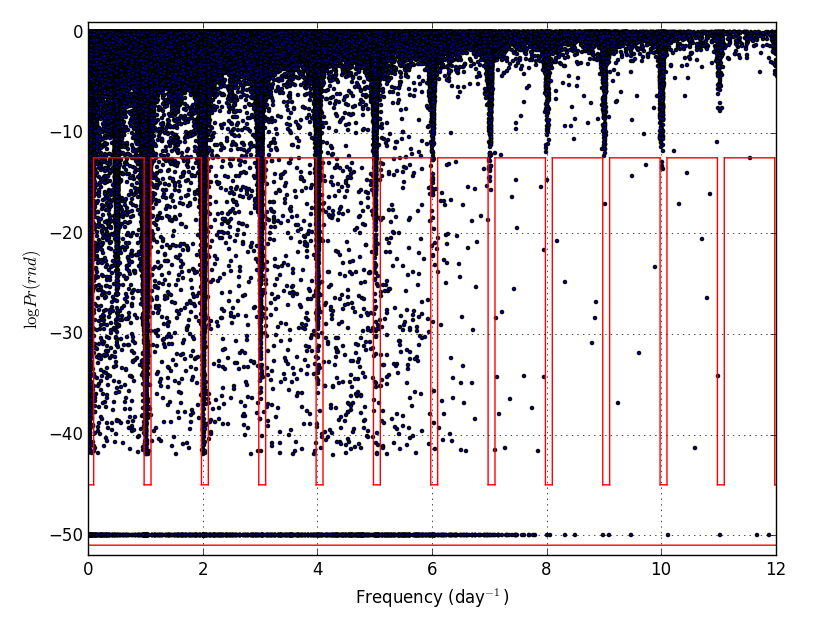
\includegraphics[width=3.3in]{figures/RlogPr.png}
 \caption{\it \small{$\log{Pr(rnd)}$ vs frequency (day$^{-1}$) of $315,992$ stars selected by the quartile criteria. The region enclosed by the red lines define the masked regions with high significance level ($\log{Pr(rnd)} < -12.5$) and no aliasing ($0.02<$ frequency $<0.98$, $1.02<$ frequency $<1.98$, etc.). The masked region contains $5,658$ stars.}} 
 \label{fig:logPr}
\end{figure}




\section{RR Lyrae Selection Criteria}

\iffalse
\begin{itemize}
	\item{} Fourier series fit to extract variable types
\end{itemize}

\begin{itemize}
	\item{} compute FS and calculate $\chi^2 / ndf$. if $\chi^2 / ndf < 10$, next step.
	\item{} find abs(max/min(FS)). if abs(max/min(FS)) $> 0.2$, then we call it's a variable stars.
	\item{} explanation of period error estimation using Fourier series.
	\end{itemize}
\fi

To identify RR Lyrae stars, we applied three criteria: gri period consistency, Fourier Sine Series $\chi^2/$ndf, and Fourier Sine Series amplitude. 

\subsection{gri Period Consistency}
The first criterion was the consistency of periods calculated by FLS from g, r, and i filters individually since RR Lyrae stars should have identically the same period in each filter in the range of $0.05$ to $1.2$~days ~\citep{Astro}. We checked whether each filter period agreed within $0.04$ days $\simeq 1$ hour with each other. 

\subsection{Fourier Sine Series $\chi^2/$ndf}
The second criterion was $\chi^2/$ndf calculated using the Fourier Sine Series (FSS). Since the RR Lyrae light curves are more or less sinusoidal, FSS with a few terms should be able to represent the light curves for certain accuracy. We used FSS in the form;

\begin{equation}
\label{FSS}
\text{FSS} = \sum_{n=1}^{N} \sin{\left(\frac{n \pi t}{P} + \phi_n \right)}
\end{equation}

\noindent where $P$ is the calculated period from FLS, $\phi_n$ is the phase, and $N$ of up to $6$ (for larger $N$, the computations were unstable; huge errors in the parameter estimations). We required the $\chi^2/$ndf be within sigma deviation of $3$, so $\chi^2/$ndf $\sim \sigma^2 < 9$. 

\subsection{Fourier Sine Series amplitude}
The third criterion was the amplitude of FSS. As mentioned before, the amplitude range of RR Lyrae stars is $0.3$ to $2.0$ mags, so we set the amplitude ranges of FSS to be $0.15$ to $2.15$ mags by taking $10\%$ photometry into account ($1.5\sigma$ limit). The four major types of RR Lyrae found by using out criteria are show in FIG. \ref{fig:Type}. The three criteria yielded $1,239$ RR Lyrae stars out of $5,658$ candidates in the masked region.


\begin{figure*}
	\centering
	\begin{subfigure}{.5\textwidth}
	  \centering
	  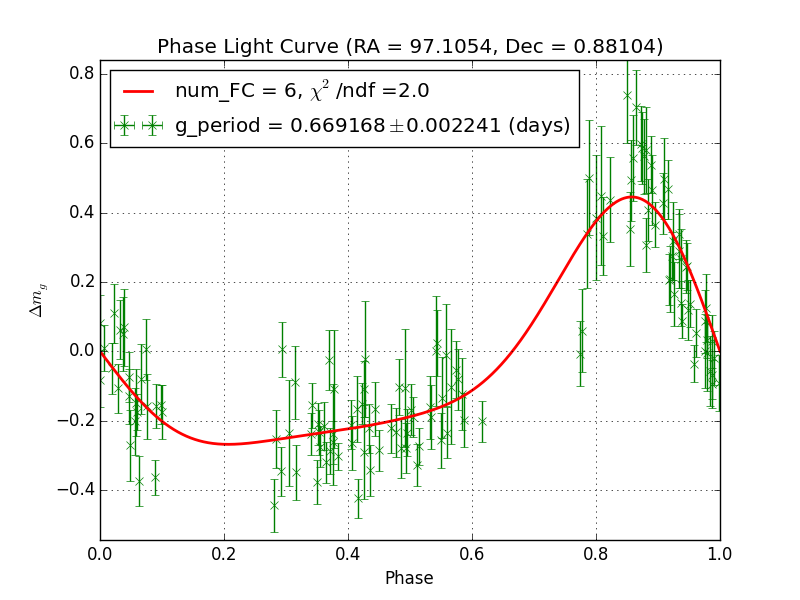
\includegraphics[width=3.35in]{figures/FSP1_g_LC_rrrtest_p5_grp19.png}
		\caption{\it \small{Type ab}}
		\label{fig:Tab}
	\end{subfigure}%
	\begin{subfigure}{.5\textwidth}
	  \centering
			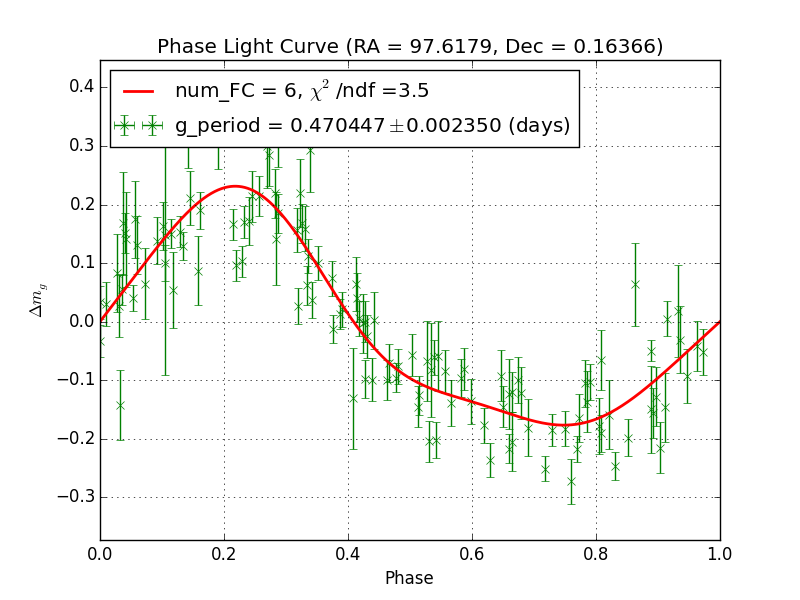
\includegraphics[width=3.35in]{figures/FSP1_g_LC_rrrtest_p5_grp7.png}
		\caption{\it \small{Type c}}
		\label{fig:Tc}
	\end{subfigure}%
	
	\begin{subfigure}{.5\textwidth}
	  \centering
			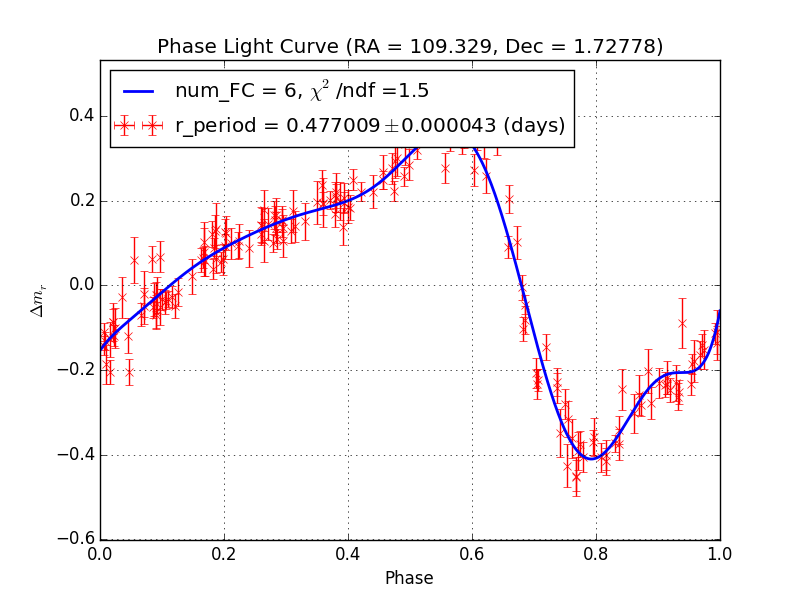
\includegraphics[width=3.35in]{figures/rPLCneg45E_limit2_grp_109+01_09693.png}
		\caption{\it \small{Blazhko Modulated \citep{RRLyrae}}}
		\label{fig:Tc}
	\end{subfigure}%
	\begin{subfigure}{.5\textwidth}
	  \centering
			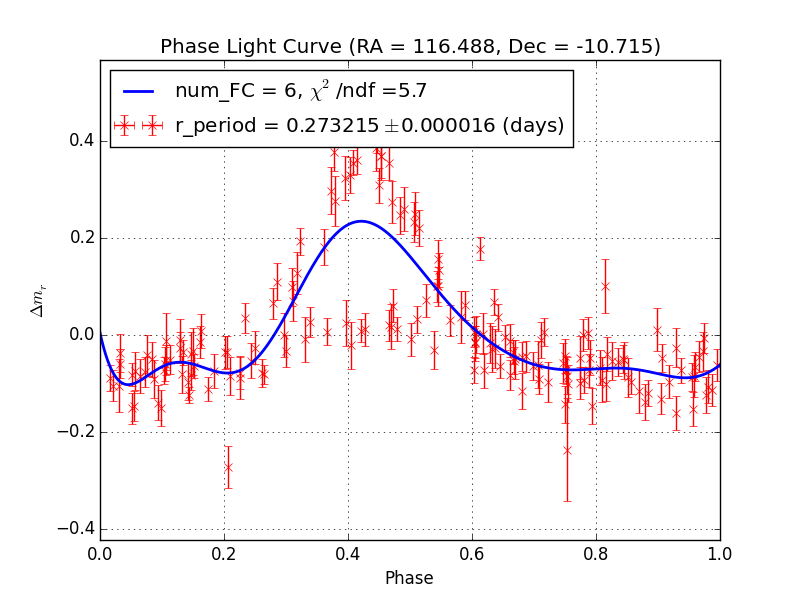
\includegraphics[width=3.35in]{figures/rPLCneg45E_limit2_grp_116-11_03117.png}
		\caption{\it \small{Period Doubling}}
		\label{fig:Tc}
	\end{subfigure}%
	\caption{\it \small{Four major types of RR Lyrae phase light curves.}}
	\label{fig:Type}
\end{figure*}


	
\subsection{Period Error Estimation}

Assuming the Gaussian statistics and Taylor expanding $\chi^2$ with respect to angular frequency, the estimated error model for angular frequency, $\delta \omega$, was constructed~\citep{gri} and expressed as;

\begin{equation}
\label{AFEE}
1 = \frac{\chi^2(\omega)}{\text{ndf}} - \frac{\chi^2(\omega_0)}{\text{ndf}} \simeq \frac{A^2}{2} \delta \omega^2 \sum_{i=1}^{\text{ndp}} \frac{(t_i - \bar{t})^2}{\delta m^2_i}
\end{equation}

\noindent where $\omega_0$ is the calculated angular frequency by FLS, $A$ is the calculated amplitude by FSS, ndp is the number of data points, $\bar{t}$ is our mean observation Julian Date, and $\delta m$ is the uncertainty in magnitude. The choice of time origin was tricky since the model allows arbitrary time origin, so we used $\bar{t}$ as a reasonable choice. Then the period uncertainties were estimated as;


\begin{equation}
\label{PEE}
\delta P = \frac{d}{d\omega} \left(\frac{2\pi}{\omega} \right) = \frac{2\pi}{\omega^2} \delta \omega \, .
\end{equation}


\section{Distance Calculations}

In order to calculate distances to RR Lyrae stars, we needed to classify RR Lyrae subtypes as shown in FIG. \ref{fig:Type}. However, there is currently only few systematic studies (calibrations) of the type classification using light curves only (mainly on types ab and c), and they are complicated in general. To avoid the complications for the moment, we used the typical absolute RR Lyrae magnitude~\citep{PSdata}, $M_r \simeq M_v = 0.6$. To estimate the amount of dust reddening, we used the total to selective extinction~\citep{Rv}, $Rv=3.1$, and the number fraction weighted average color term~\citep{EBV}, $(B-V)_0 = 0.358$, of RRab and RRc stars. The number fraction weighted average $(B-V)_0$ was calculated by using the number statistics of known RR Lyrae stars ($\simeq91\%$ of RR Lyares are type ab and $\simeq9\%$ of RR Lyraes are type c assuming that the numbers of Blazhko modulated and period doubling are negligible) as follows;

\begin{equation}
\label{BV}
(B-V)_0 = 0.91(B-V)_{ab0} + 0.09(B-V)_{c0}
\end{equation}

\noindent where $(B-V)_{ab0} \simeq 0.372$ and $(B-V)_{c0} \simeq 0.211$. Then the color extinction was calculated as~\cite{Modern};

\begin{equation}
\label{EBV}
E(B-V) = (B-V)_{observed} - (B-V)_0 \, ,
\end{equation}

\noindent and the extinction was calculated as~\cite{Modern};

\begin{equation}
\label{Av}
A_v = R_v E(B-V) \,
\end{equation}

\noindent Finally, the distance was calculated by using the distance modulus;

\begin{equation}
\label{dist}
d = 10^{[1+(m_r - A_v - M_v)/5]} \, .
\end{equation}

\noindent To convert the gri magnitudes to the Johnson magnitudes, the conversions given by the Sloan Digital Sky Survey (SDSS)~\cite{SDSS} were used.

\section{Results}
\begin{itemize}
	\item{} compare with PS~\cite{PSdata}
	\item{} density/distribution of variables in sky
	\item{} (what LS gave us for our catalog)
	\item{} put a table with ~5 stars, to show off part of catalog
\end{itemize}




\subsection{Spatial Distributions}

From the calculated distances, the distance histogram of RR Lyrae stars is plotted and shown in FIG. \ref{fig:dhist}. It almost follows the Gaussian distribution. The spatial distributions and histograms of RR Lyrae stars are shown in  FIG. \ref{fig:RRspace} and \ref{fig:blhist}, respectively. As in FIG. \ref{fig:RRspace}, 

\begin{figure}[H]
 \centering
 	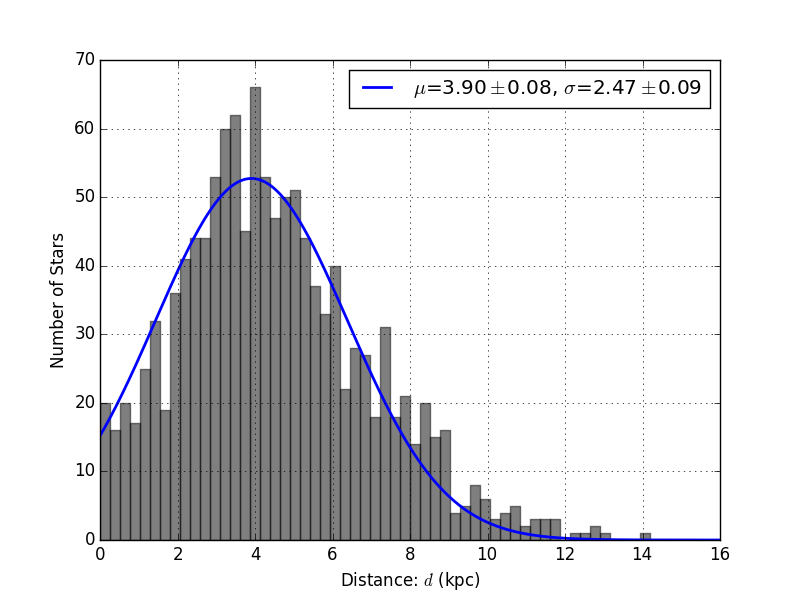
\includegraphics[width=3.3in]{figures/PlotsSpace15/gdhist_limit15.png}
 \caption{\it \small{Distance histograms of 1,239 RR Lyrae stars with a Gaussian fit. The Gaussian fit was used to aid for seeing the general radial distribution of RR Lyrae stars. }} 
 \label{fig:dhist}
\end{figure} 


\begin{figure*}
	\centering
	\begin{subfigure}{.5\textwidth}
	  \centering
	  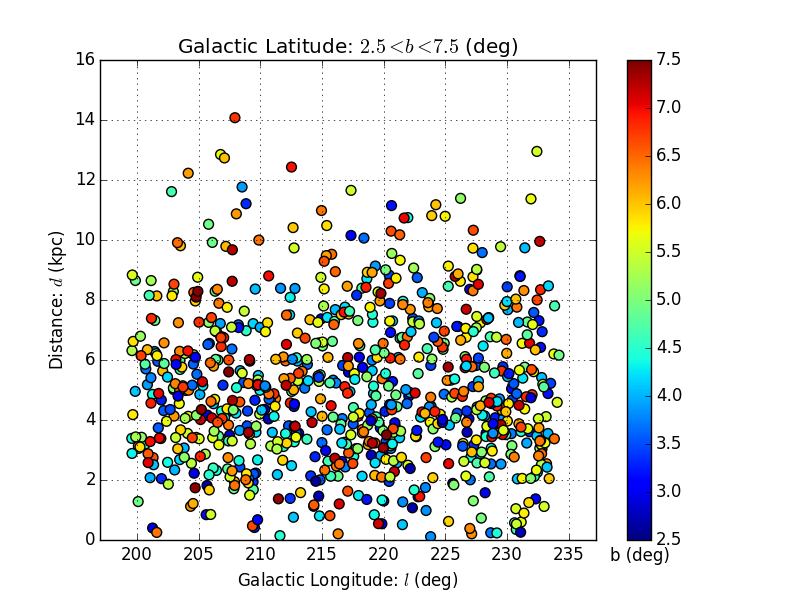
\includegraphics[width=3.35in]{figures/PlotsSpace15/dist_b_lp_limit15.png}
		\caption{\it \small{$2.5 < b < 7.5$ }}
		\label{fig:blp}
	\end{subfigure}%
	\begin{subfigure}{.5\textwidth}
	  \centering
			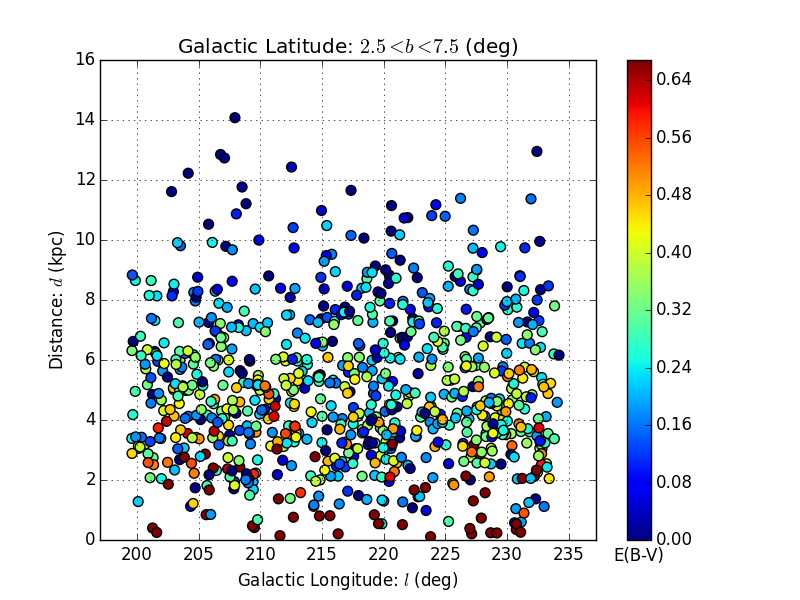
\includegraphics[width=3.35in]{figures/PlotsSpace15/dist_EBV_lp_limit15.png}
		\caption{\it \small{$E(B-V)$ for $2.5 < b < 7.5$ }}
		\label{fig:EBVlp}
	\end{subfigure}%
	
	\begin{subfigure}{.5\textwidth}
	  \centering
			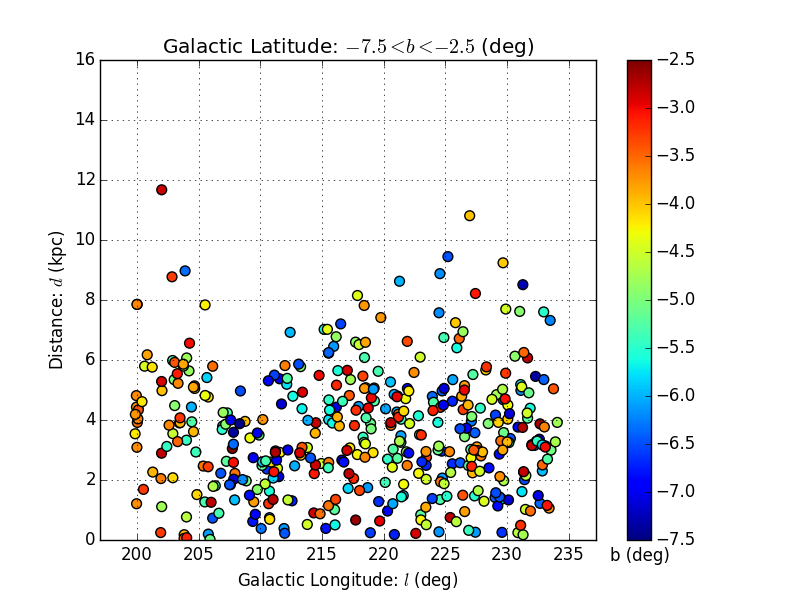
\includegraphics[width=3.35in]{figures/PlotsSpace15/dist_b_ln_limit15.png}
		\caption{\it \small{$-7.5 < b < -2.5$ }}
		\label{fig:bln}
	\end{subfigure}%
	\begin{subfigure}{.5\textwidth}
	  \centering
			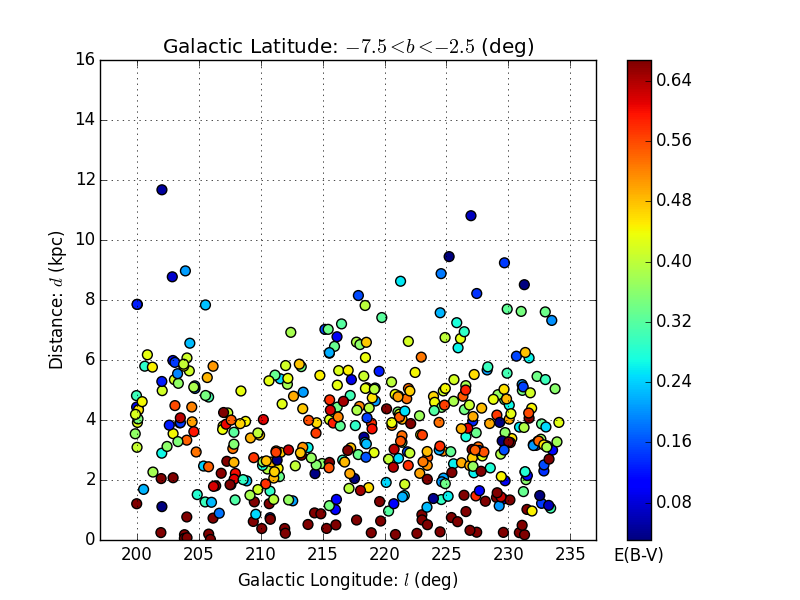
\includegraphics[width=3.35in]{figures/PlotsSpace15/dist_EBV_ln_limit15.png}
		\caption{\it \small{$E(B-V)$ for $-7.5 < b < -2.5$ }}
		\label{fig:EBVln}
	\end{subfigure}%
	\caption{\it \small{Spatial distributions of 1,239 RR Lyrae stars. The galactic longitude and latitude range correspond to our FOV. The range of $E(B-V)$ corresponds to the mean $E(B-V)$ $\pm$ $1\sigma$.}}
	\label{fig:RRspace}
\end{figure*}



\begin{figure*}
	\centering
	\begin{subfigure}{.5\textwidth}
	  \centering
	  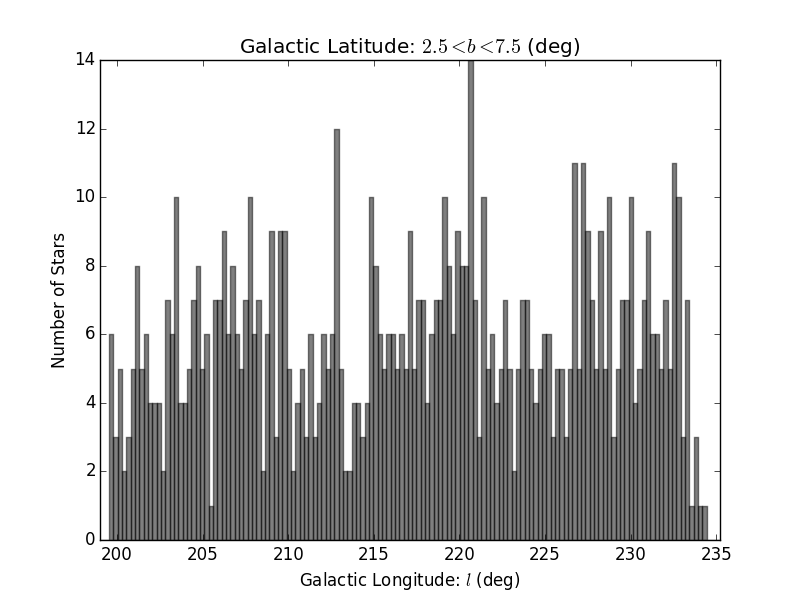
\includegraphics[width=3.35in]{figures/PlotsSpace15/lphist_limit15.png}
		\caption{\it \small{Galactic longitudinal histogram for $2.5 < b < 7.5$}}
		\label{fig:bphist}
	\end{subfigure}%
	\begin{subfigure}{.5\textwidth}
	  \centering
			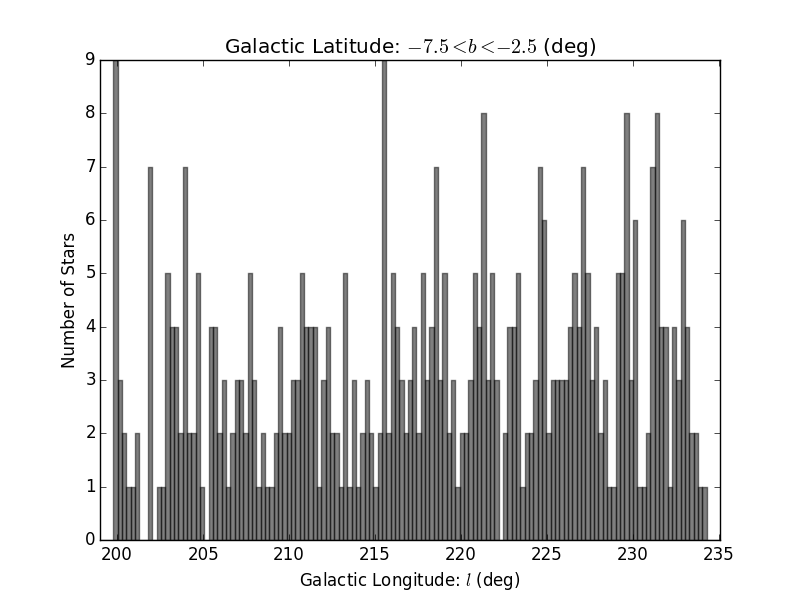
\includegraphics[width=3.35in]{figures/PlotsSpace15/lnhist_limit15.png}
		\caption{\it \small{Galactic longitudinal histogram for $-7.5 < b < -2.5$ }}
		\label{fig:bnhist}
	\end{subfigure}%
	
	\begin{subfigure}{.5\textwidth}
	  \centering
	  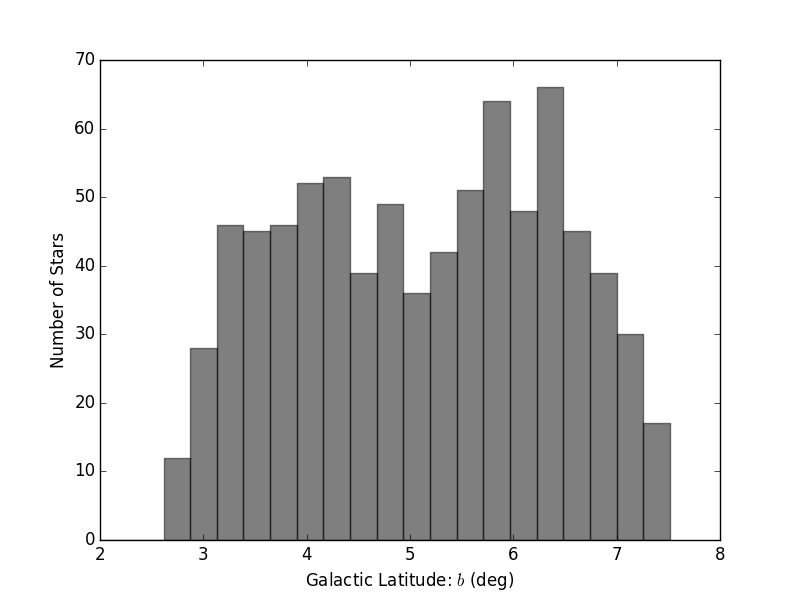
\includegraphics[width=3.35in]{figures/PlotsSpace15/bphist_limit15.png}
		\caption{\it \small{Galactic latitudinal histogram for $2.5 < b < 7.5$}}
		\label{fig:bphist}
	\end{subfigure}%
	\begin{subfigure}{.5\textwidth}
	  \centering
			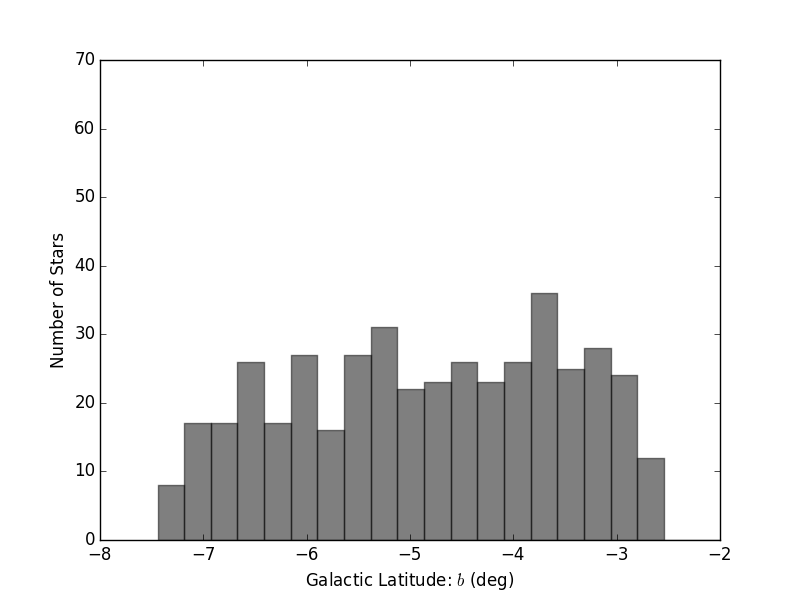
\includegraphics[width=3.35in]{figures/PlotsSpace15/bnhist_limit15.png}
		\caption{\it \small{Galactic latitudinal histogram for $-7.5 < b < -2.5$}}
		\label{fig:bnhist}
	\end{subfigure}%
	\caption{\it \small{Spatial histograms of 1,239 RR Lyrae stars. The galactic longitude and latitude range correspond to our FOV.}}
	\label{fig:blhist}
\end{figure*}

 





%\section{Evaluating the Pan-STARRS Variability Parameter}
\section{Evaluating the HPS Variability Parameter}
\begin{itemize}
%	\item{} compare with HPS~\cite{PSdata}
%	\item{} density/distribution of variables in sky
%	\item{} (what FLS gave us for our catalog)
	\item{} put a table with ~5 stars, to show off part of catalog
\end{itemize}


A paper, \textit{Finding, Characterizing and Classifying Variable Sources in Multi-Epoch Sky Surveys: QSOs and RR Lyrae in PS1 $3\pi$ Data}~\cite{PSdata} (HPS), quantifies the likelihood that a star is an RR Lyrae.  Using their variability statistic, $\rho_{RRLyrae}$, density and distribution of RR Lyrae and other variable candidates were determined.  Table~\ref{tab:HPSlim15} evaluates the validity of HPS's variability criteria.

% HPS.restrictFOV.m11.m16.chyea has 5900 stars in it --> 5900 HPS stars in our FOV
% THIS TABLE IS FOR LIMIT 0.15
\begin{table*}
%\begin{table}[H]
	\begin{center}
		\begin{tabular}{|c|c|c|c|c|c|c|c|}\hline
			%HPS stat & nonvar15 & var15 \\ \hline
HPS $\rho_{RRLyrae}$ & $HPS_{total}$ & $HPS_{matched}$ & RR Lyrae & Not RR Lyrae & Prob(RR) \\ \hline
0.0-0.05 & 5029 & 138 & 46 		& 92 & 0.33 \\ \hline
0.05-0.1 & 124 & 25 & 12 		& 13 & 0.48 \\ \hline
0.1-0.2 & 154 & 38 & 19 		& 19 & 0.50 \\ \hline
0.2-0.3 & 116 & 36 & 15 		& 21 & 0.42 \\ \hline
0.3-0.4 & 82 & 36 & 22 			& 14 & 0.61 \\ \hline
0.4-0.5 & 85 & 34 & 20			& 14 & 0.59 \\ \hline
0.5-0.6 & 90 & 41 & 22			& 19 & 0.54 \\ \hline
0.6-0.7 & 89 & 47 & 28			& 19 & 0.60 \\ \hline
0.7-0.8 & 64 & 39 & 28 			& 11 & 0.72 \\ \hline
0.8-0.9 & 46 & 28 & 23 			& 5 & 0.82 \\ \hline
0.9-1.0 & 21 & 15 & 9			& 6 & 0.60 \\ \hline
\hline
0.0-1.0 & 5900 & 477 & 244 & 233 & 0.51 \\ \hline
		\end{tabular}
	\end{center}
\caption{ \small{A comparison of verified observations and HPS RR Lyrae candidates. \label{tab:HPSlim15}}}
\end{table*}

%[46, 12, 19, 15, 22, 20, 22, 28, 28, 23, 9, 0]


Figure~\ref{fig:probrrHPS} shows no correlation between the HPS criteria and candidates verified to be RR Lyrae stars.  Of the 1.5 Billion stars identified in our FOV, we isolated the 320,000 most variable, 
%using the lower quartile variance, as described in~\cref{sec:cuts}.
as described in~\cref{sec:cuts}.


%The further a star lands from a linear fit to this plot, the higher probability it is variable.  
%~[DESCRIBE LOWER QUARTILE METHOD]
%The star (group) histogram counts have a massive peak around 110 (g), 140 (r) and 125 (i), with low count peaks at N<50.
%Picking N>100 doesn't look like it misses many real stars.
%The plot of quartile variance in realstar.? (col 11-10 vs col 9) shows a 
%flattening out at g<13, and then increase by Poisson as 0.2*m Sort these in order of decreasing variability


A grouping and matching algorithm, written by J. Tonry~\cite{gri}, made it possible to isolate and group 
stars from various nights of observations.  
Implementation of logPr(rnd) allowed for complete confirmation of RR Lyrae candidates.  Only stars with different 
variable classifications, those having lower amplitude variations, would have been able to go
undetected.  Masking out regions of high aliasing reduced the need to run a more rigorous analysis, % of variable candidates,  
due to the statistically improbability of these sources being variable.  A total of 5,658 stars fell within 
the masked region, shown in Figure~\ref{RlogPr.png}.  FLS and FSS analysis identified 1,239 variable stars in our FOV.  
A defining characteristic of RR Lyrae is their variability periods, falling between 0.5 and 1.2 days.  Using this 
restriction 279 stars were confirmed to be RR Lyrae.  Variability classification was confirmed by visually inspecting 
the light curves of all 279 RR Lyrae and the remaining 960 unclassified variable stars.  Following this procedure gives us 
$100\%$ purity.

\begin{figure}[H]
 \centering
 	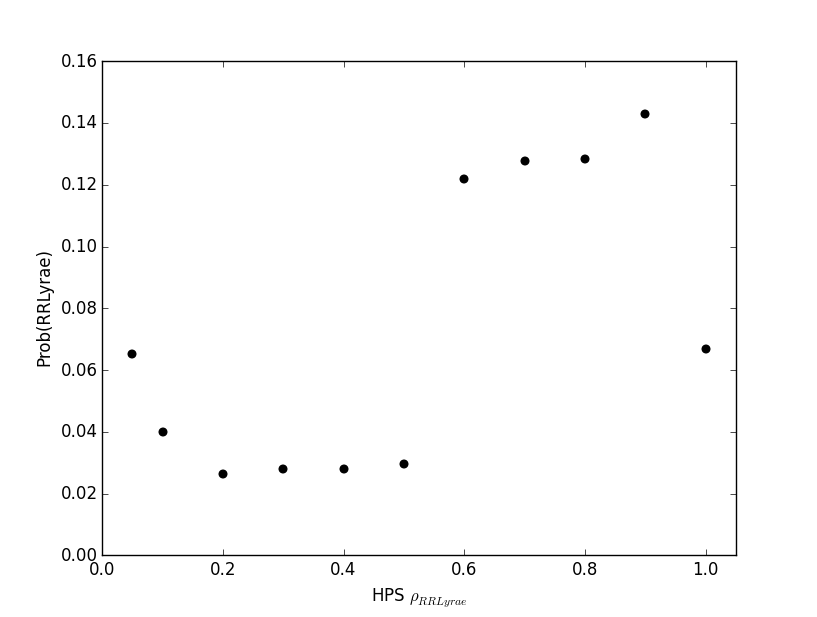
\includegraphics[width=3.35in]{figures/probrr_vs_HPS.png}
 \caption{\it \small{Evaluation of HPS RR Lyrae criteria.}}
 \label{fig:probrrHPS}
\end{figure}

Using the same matching algorithm~\cite{gri} made comparing observations with other variable catalogs possible.  
To evaluate the HPS RR Lyrae criteria, our observations were matched to stars flagged as potential RR Lyrae candidates by HPS.  
Shown in Table~\ref{tab:HPSlim15} and Figure~\ref{fig:probrrHPS}, there is no correlation between HPS criteria and 
verified RR Lyrae stars.









\section{Discussion}
\iffalse
\begin{itemize}
	\item{} Evaluation of PS criteria
	\item{} what went wrong
	\item{} what could have gone better
	\item{} future outlook
	\item{}~~~we could map spiral arms using x y and z
\end{itemize}
\fi

In order to evaluate the completeness of our results, comparisons needed to be made to other variable star catalogs.  Simbad~\cite{simbad} provided a list of variable stars within our FOV.  Pulsating sources encompasses all variable objects.  With 48 objects overlapping our FOV, shown in Figure~\ref{fig:simoverlap}, we achieved a completeness of $98\%$.

~[possible put two light curves in as examples of objects that overlap our field]\\

\begin{figure}[H]
 \centering
 %\caption{prob(f)}
 %\textbf{Simbad Completeness}\par\medskip
 	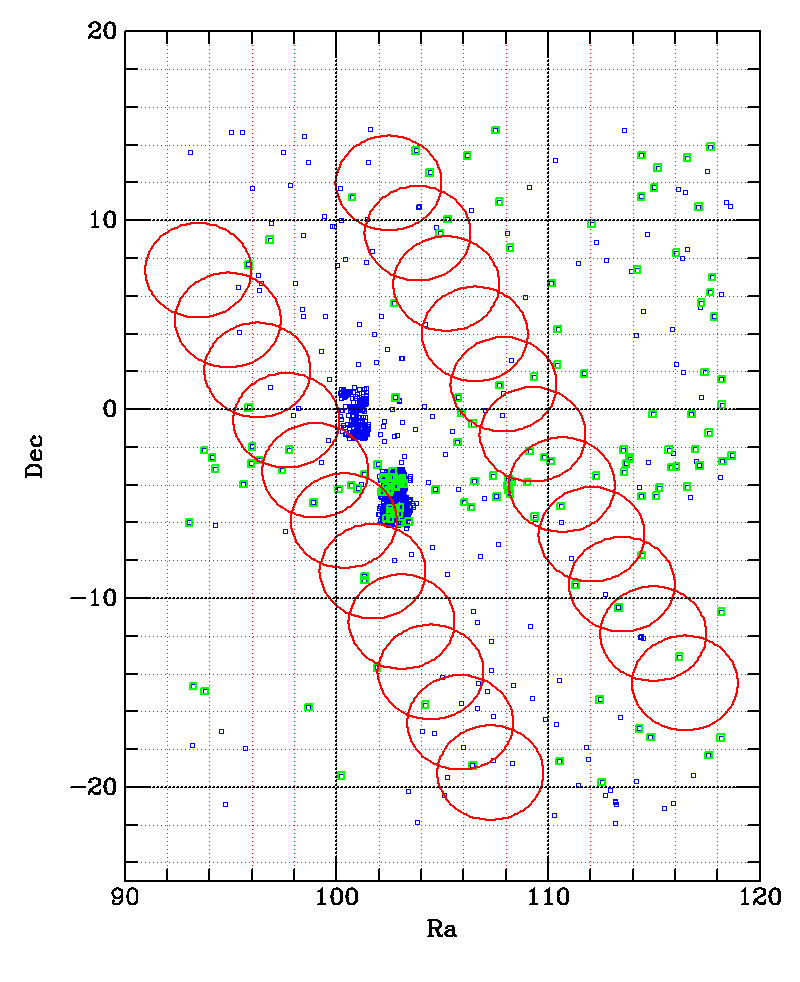
\includegraphics[width=3.35in]{figures/simbadoverlap.png}
 \caption{\it \small{Observation path shown in red, with Simbad pulsators in blue and RR Lyrae in green.}}
 \label{fig:simoverlap}
\end{figure}


%\begin{figure}[h!]
%	\centering
%	\begin{subfigure}{.5\textwidth}
%	  \centering
%	  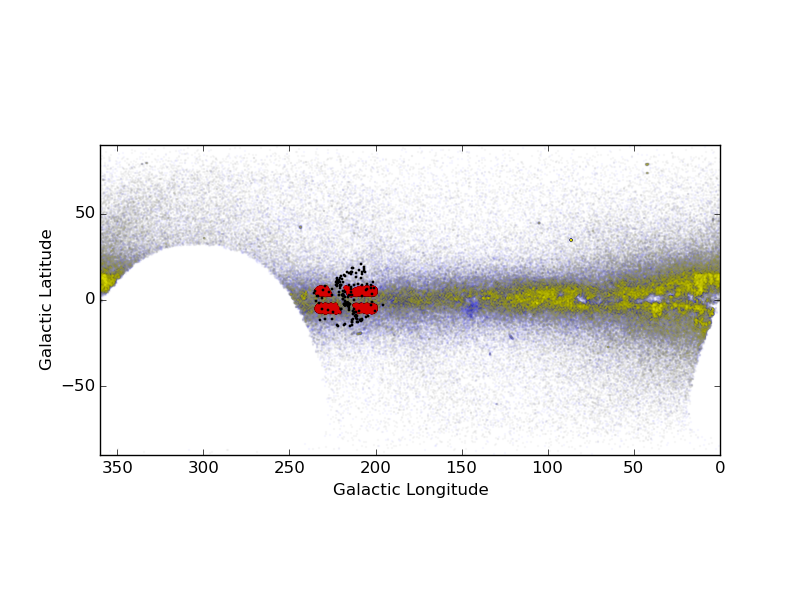
\includegraphics[width=1\linewidth]{figures/aitoff/simbad_alpha_is_1.png}
%	  \caption{\it \small{Aitoff map.}}
%	  \label{fig:aitoff_map_simbad}
%	\end{subfigure}%
%	\begin{subfigure}{.5\textwidth}
%	  \centering
%	  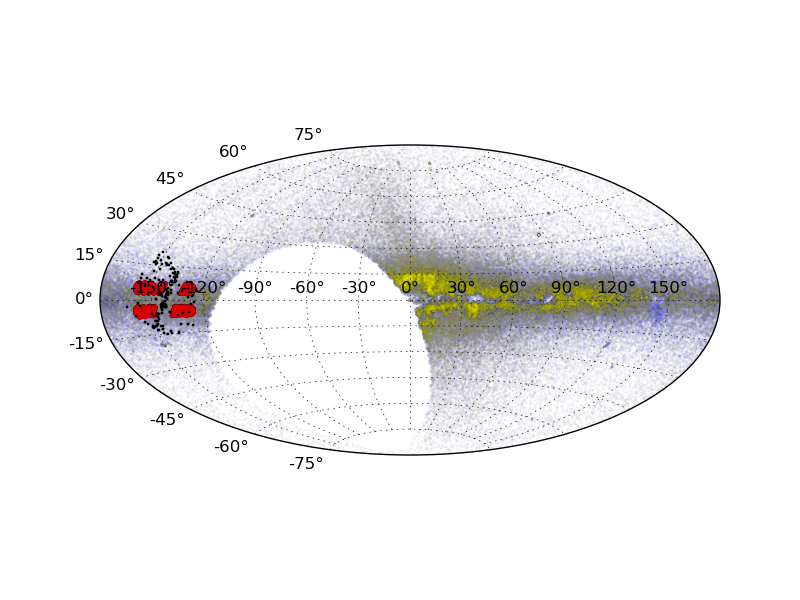
\includegraphics[width=1\linewidth]{figures/aitoff/Obs_PS_sim_lsum_aitoff_map.png}
%	 \caption{\it \small{Aitoff projection}}%
%	 \label{fig:aitoff_projection_simbad}
%	\end{subfigure}
%	\caption{\it \small{Aitoff projection of observed and PS RR Lyrae candidates.  Blue are candidates from PS that >= 0.05, yellow are PS candidates that >= 0.2., observed data in red, simbad in black.}}
%	\label{fig:aitoff_simbad}
%\end{figure}	


\section{Summary and Conclusions}
~[TALK ABOUT IT]


%\section{Resources from website (remove this section)}
%\begin{itemize}
%	\item{} $ay301.ifa.hawaii.edu$
%	\item{} $/ay301/atlas = location for all the gri Project data and programs$
%	\item{} $/ay301/script = transcripts from class computer activities$
%	\item{} $/ay301/tmp = generic temporary area$
%	\item{} $gri Project$
%	\item{} $/home/gri_project = location for manuscript and figures$
%	\item{} $Las Cumbres LCOGT (Faulkes 2m telescope on Haleakala)$
%	\item{} $ATLAS (fallingstar.com)$
%	\item{} $0.5m telescope with c,o,B,V,R,I,H-alpha filters$
%	\item{} $0.18m Pathfinder telescope with g,r,i filters$
%	\item{} $0.06m 35mm piggy-back camera with RGB$
%	\item{} $0.01m 35mm fisheye camera$
%\end{itemize}


\section*{Acknowledgments}
We would like to thank \input acknowledgement.tex  % input acknowledgement





\setlength{\parindent}{0cm}

\bibliography{biblio}


%\begin{thebibliography}{99}  % the trailing 99 controls some obscure format--just use	
%~\\% needed for spacing	
%\bibitem{PSimgpipe} Magnier E 2006 The Pan-STARRS PS1 image processing pipeline. In \textit{Proceedings of the Advanced Maui Optical and Space Surveillance Technologies Conf.} (ed. Ryan S), \textit{Wailea, Maui, HI, 10–14 September 2006,} p. E5. Kihei, HI: The Maui Economic Development Board.\\	
%\bibitem{simbad} Simbad Database	
%\bibitem{tonrypipe} Tonry JL, et al. 2012 The Pan-STARRS1 photometric system. \textit{Astrophys. J.} \textbf{750}, 99. doi:10.1088/0004-637X/750/2/99\\	
%\bibitem{gri} Tonry JL, er al. 2016 (personal communications January-April 2016)\\	
%\end{thebibliography}


\end{document}

